% Options for packages loaded elsewhere
\PassOptionsToPackage{unicode}{hyperref}
\PassOptionsToPackage{hyphens}{url}
\PassOptionsToPackage{dvipsnames,svgnames,x11names}{xcolor}
%
\documentclass[
  10pt,
  ignorenonframetext,
]{beamer}
\usepackage{pgfpages}
\setbeamertemplate{caption}[numbered]
\setbeamertemplate{caption label separator}{: }
\setbeamercolor{caption name}{fg=normal text.fg}
\beamertemplatenavigationsymbolsempty
% Prevent slide breaks in the middle of a paragraph
\widowpenalties 1 10000
\raggedbottom
\setbeamertemplate{part page}{
  \centering
  \begin{beamercolorbox}[sep=16pt,center]{part title}
    \usebeamerfont{part title}\insertpart\par
  \end{beamercolorbox}
}
\setbeamertemplate{section page}{
  \centering
  \begin{beamercolorbox}[sep=12pt,center]{part title}
    \usebeamerfont{section title}\insertsection\par
  \end{beamercolorbox}
}
\setbeamertemplate{subsection page}{
  \centering
  \begin{beamercolorbox}[sep=8pt,center]{part title}
    \usebeamerfont{subsection title}\insertsubsection\par
  \end{beamercolorbox}
}
\AtBeginPart{
  \frame{\partpage}
}
\AtBeginSection{
  \ifbibliography
  \else
    \frame{\sectionpage}
  \fi
}
\AtBeginSubsection{
  \frame{\subsectionpage}
}
\usepackage{amsmath,amssymb}
\usepackage{lmodern}
\usepackage{iftex}
\ifPDFTeX
  \usepackage[T1]{fontenc}
  \usepackage[utf8]{inputenc}
  \usepackage{textcomp} % provide euro and other symbols
\else % if luatex or xetex
  \usepackage{unicode-math}
  \defaultfontfeatures{Scale=MatchLowercase}
  \defaultfontfeatures[\rmfamily]{Ligatures=TeX,Scale=1}
\fi
\usetheme[]{Singapore}
\usefonttheme{serif}
% Use upquote if available, for straight quotes in verbatim environments
\IfFileExists{upquote.sty}{\usepackage{upquote}}{}
\IfFileExists{microtype.sty}{% use microtype if available
  \usepackage[]{microtype}
  \UseMicrotypeSet[protrusion]{basicmath} % disable protrusion for tt fonts
}{}
\makeatletter
\@ifundefined{KOMAClassName}{% if non-KOMA class
  \IfFileExists{parskip.sty}{%
    \usepackage{parskip}
  }{% else
    \setlength{\parindent}{0pt}
    \setlength{\parskip}{6pt plus 2pt minus 1pt}}
}{% if KOMA class
  \KOMAoptions{parskip=half}}
\makeatother
\usepackage{xcolor}
\newif\ifbibliography
\usepackage{graphicx}
\makeatletter
\def\maxwidth{\ifdim\Gin@nat@width>\linewidth\linewidth\else\Gin@nat@width\fi}
\def\maxheight{\ifdim\Gin@nat@height>\textheight\textheight\else\Gin@nat@height\fi}
\makeatother
% Scale images if necessary, so that they will not overflow the page
% margins by default, and it is still possible to overwrite the defaults
% using explicit options in \includegraphics[width, height, ...]{}
\setkeys{Gin}{width=\maxwidth,height=\maxheight,keepaspectratio}
% Set default figure placement to htbp
\makeatletter
\def\fps@figure{htbp}
\makeatother
\setlength{\emergencystretch}{3em} % prevent overfull lines
\providecommand{\tightlist}{%
  \setlength{\itemsep}{0pt}\setlength{\parskip}{0pt}}
\setcounter{secnumdepth}{-\maxdimen} % remove section numbering
\newlength{\cslhangindent}
\setlength{\cslhangindent}{1.5em}
\newlength{\csllabelwidth}
\setlength{\csllabelwidth}{3em}
\newlength{\cslentryspacingunit} % times entry-spacing
\setlength{\cslentryspacingunit}{\parskip}
\newenvironment{CSLReferences}[2] % #1 hanging-ident, #2 entry spacing
 {% don't indent paragraphs
  \setlength{\parindent}{0pt}
  % turn on hanging indent if param 1 is 1
  \ifodd #1
  \let\oldpar\par
  \def\par{\hangindent=\cslhangindent\oldpar}
  \fi
  % set entry spacing
  \setlength{\parskip}{#2\cslentryspacingunit}
 }%
 {}
\usepackage{calc}
\newcommand{\CSLBlock}[1]{#1\hfill\break}
\newcommand{\CSLLeftMargin}[1]{\parbox[t]{\csllabelwidth}{#1}}
\newcommand{\CSLRightInline}[1]{\parbox[t]{\linewidth - \csllabelwidth}{#1}\break}
\newcommand{\CSLIndent}[1]{\hspace{\cslhangindent}#1}
\setbeamertemplate{navigation symbols}{}
\setbeamertemplate{footline}[page number]
\ifLuaTeX
  \usepackage{selnolig}  % disable illegal ligatures
\fi
\IfFileExists{bookmark.sty}{\usepackage{bookmark}}{\usepackage{hyperref}}
\IfFileExists{xurl.sty}{\usepackage{xurl}}{} % add URL line breaks if available
\urlstyle{same} % disable monospaced font for URLs
\hypersetup{
  pdftitle={Best practices for reporting scientific results},
  pdfauthor={Stefanie Muff},
  colorlinks=true,
  linkcolor={Maroon},
  filecolor={Maroon},
  citecolor={Blue},
  urlcolor={blue},
  pdfcreator={LaTeX via pandoc}}

\title{Best practices for reporting scientific results}
\subtitle{Navigating the minefield around \(P\)-values and significance}
\author{Stefanie Muff}
\date{Open Science course, Finse, November 2022}

\begin{document}
\frame{\titlepage}

\begin{frame}
\begin{block}{The ongoing controversy around \(p\)-values}
\protect\hypertarget{the-ongoing-controversy-around-p-values}{}
\(~\)

\centering

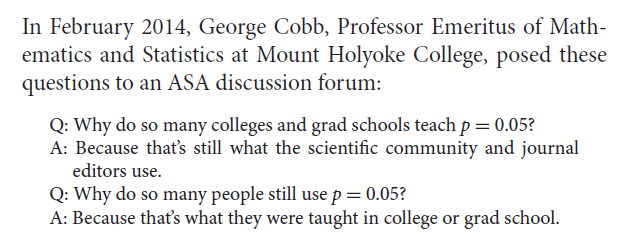
\includegraphics[width=0.9\textwidth,height=\textheight]{graphics/pvalue_circle.png}

\(~\)

\flushleft
\scriptsize

(Wasserstein and Lazar 2016)
\end{block}
\end{frame}

\begin{frame}
\begin{block}{Lots of publications in the past decades\ldots{}}
\protect\hypertarget{lots-of-publications-in-the-past-decades}{}
\(~\)


\includegraphics[width=0.5\textwidth,height=\textheight]{graphics/nuzzo.png}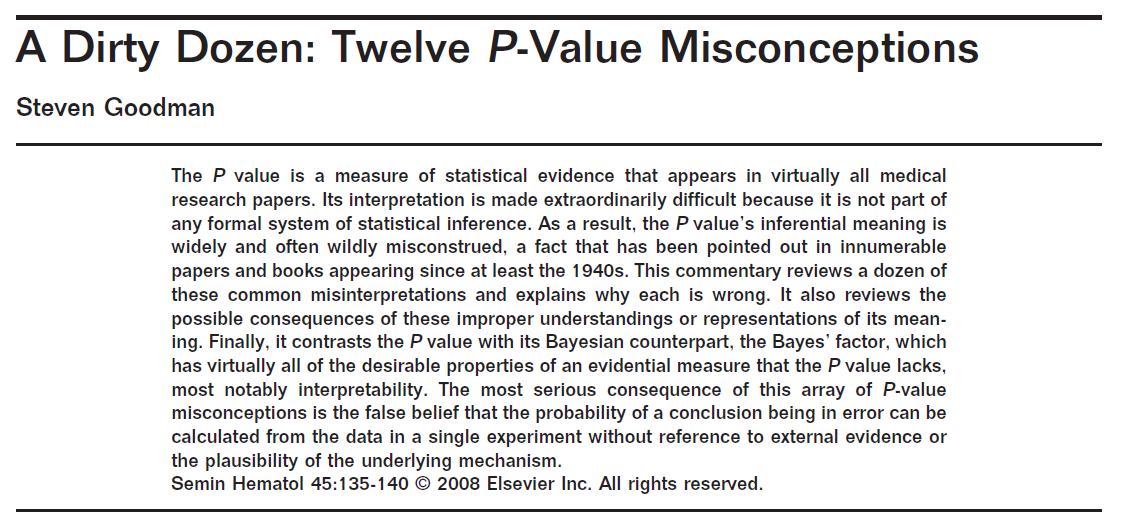
\includegraphics[width=0.5\textwidth,height=\textheight]{graphics/dirtydozen.png}

\includegraphics[width=0.5\textwidth,height=\textheight]{graphics/against_ss.png}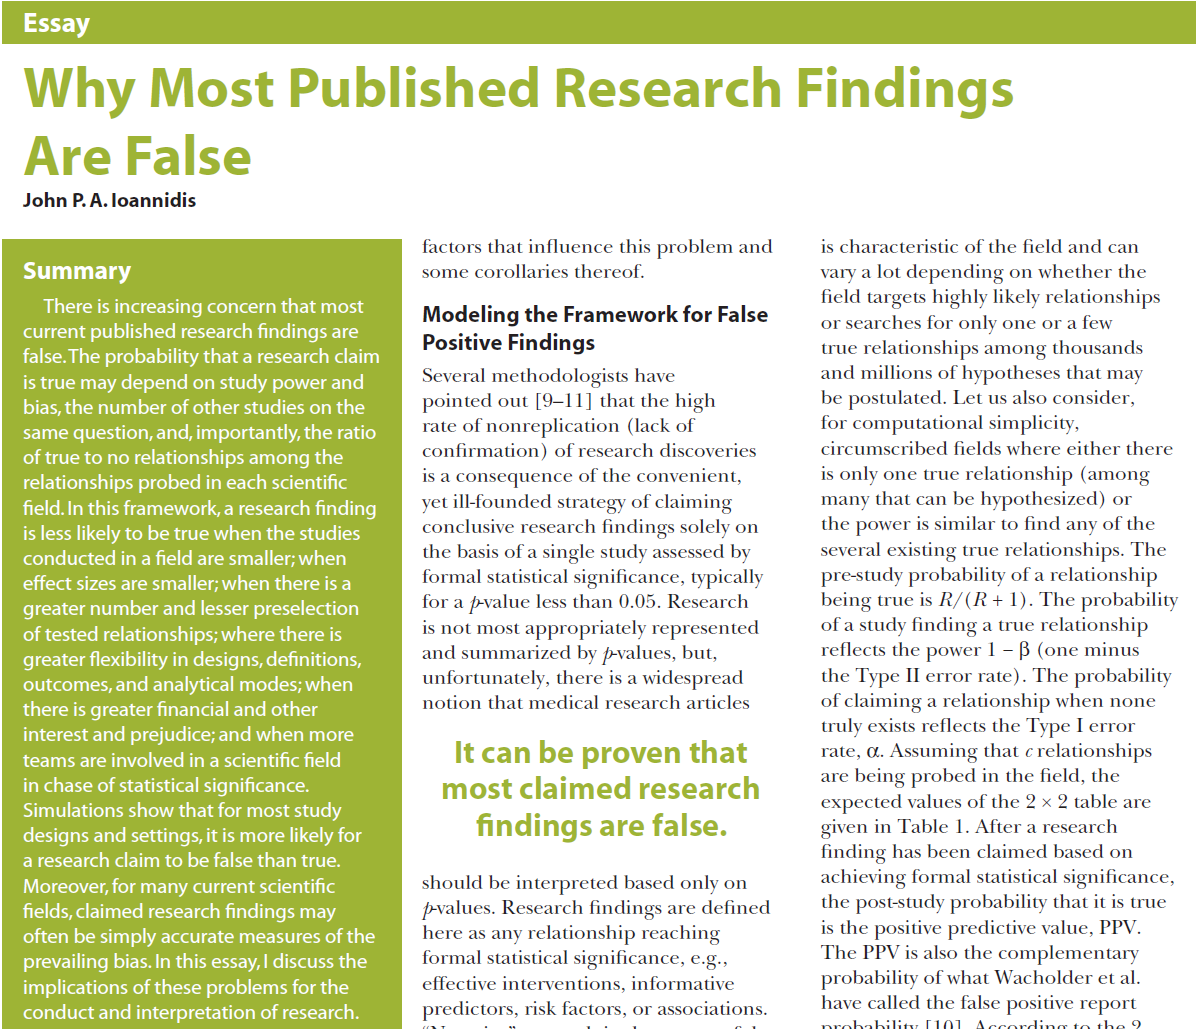
\includegraphics[width=0.4\textwidth,height=\textheight]{graphics/Ioannidis2.png}

\(~\)

\scriptsize

Ioannidis (2005), Goodman (2008), Nuzzo (2014), Amrhein, Greenland, and
McShane (2019), \ldots{}
\end{block}
\end{frame}

\begin{frame}
\begin{block}{\(P\)-values / statistical significance criticism}
\protect\hypertarget{p-values-statistical-significance-criticism}{}
\(~\)

\(P\)-value \textbf{criticism is} as \textbf{old} as statistical
significance testing (1920s!). Issues:

\(~\)

\begin{itemize}
\tightlist
\item
  The sharp line \(p<0.05\) is \emph{arbitrary}.
\end{itemize}

\(~\)

\begin{itemize}
\tightlist
\item
  \(P\)-hacking / data dredging: Search until you find a result with
  \(p<0.05\).
\end{itemize}

\(~\)

\begin{itemize}
\tightlist
\item
  Publication bias: Studies with \(p<0.05\) are more likely to be
  published than ``non-significant'\,' results.
\end{itemize}

\(~\)

\begin{itemize}
\tightlist
\item
  HARKING: Hypothesizing After the Results are Known.
\end{itemize}

\(~\)

\begin{itemize}
\tightlist
\item
  Model selection using \(p\)-values \(\rightarrow\) \textbf{model
  selection bias}.
\end{itemize}
\end{block}
\end{frame}

\begin{frame}
Note: R.A. Fisher, the ``inventor'' of the \(p\)-value (1920s) didn't
mean the \(p\)-value to be used in the way it is used today, which is:
doing a single experiment and use \(p<0.05\) for a conclusion.

\(~\)

From Goodman (2016):

\(~\)

\begin{quote}
Fisher used ``significance'' merely \textbf{to indicate that an
observation was worth following up, with refutation of the null
hypothesis justified only if further experiments ``rarely failed'' to
achieve significance}. This is in stark contrast to the modern practice
of making claims based on a single demonstration of statistical
significance.
\end{quote}

\(~\)

\pause

\centering
\end{frame}

\begin{frame}
\begin{block}{Right or wrong?}
\protect\hypertarget{right-or-wrong}{}
\(~\)

Go to www.menti.com and use code 3944 9342.

Which of these statements are right or wrong?

\(~\)

\begin{enumerate}
\tightlist
\item
  The \(p\)-value is the probability that the null hypothesis is true.
\end{enumerate}

\vspace{2mm}

\begin{enumerate}
\setcounter{enumi}{1}
\tightlist
\item
  \(p=0.02\) means that the alternative hypothesis is true with 98\%
  probability.
\end{enumerate}

\vspace{2mm}

\begin{enumerate}
\setcounter{enumi}{2}
\tightlist
\item
  The \(p\)-value is the type-1 error rate.
\end{enumerate}

\vspace{2mm}

\begin{enumerate}
\setcounter{enumi}{3}
\tightlist
\item
  The \(p\)-value is the probability that the result happened by chance.
\end{enumerate}

\vspace{2mm}

\begin{enumerate}
\setcounter{enumi}{4}
\tightlist
\item
  If \(p>0.05\), we can conclude that there is no effect.
\end{enumerate}

\vspace{2mm}

\begin{enumerate}
\setcounter{enumi}{5}
\tightlist
\item
  Two studies with \(p>0.05\) and \(p<0.05\) are in a conflict.
\end{enumerate}

\vspace{7mm}
\end{block}
\end{frame}

\begin{frame}
\begin{block}{Significance thresholding is arbitrary}
\protect\hypertarget{significance-thresholding-is-arbitrary}{}
\(~\)

\begin{itemize}
\tightlist
\item
  Is there a significant difference between \(p=0.049\) and
  \(p=0.051\)\ldots??
\end{itemize}

\pause
\vspace{2mm}

\begin{quote}
\textbf{No: }
\textcolor{red}{The difference between significant and non-significant is not necessarily significant.}
\end{quote}

\vspace{2mm}

\pause

\begin{itemize}
\tightlist
\item
  Does \(p>0.05\) automatically imply that a variable is unimportant or
  that it has no effect?
\end{itemize}

\pause
\vspace{2mm}

\begin{quote}
\textbf{No}:
\textcolor{red}{Absence of evidence is not evidence of absence} (Altman
and Bland 1995). \textcolor{red}{The null hypothesis cannot be proved.}
\end{quote}

\pause

\(~\)

Reasons for large \(p\)-values:

\begin{itemize}
\tightlist
\item
  Low sample size (\(\rightarrow\) low power).
\item
  The truth is not far from the null hypothesis.
\item
  Collinear covariates.
\end{itemize}
\end{block}
\end{frame}

\begin{frame}
\(~\)

\begin{itemize}
\tightlist
\item
  ``Statistical significance'' is often used almost synonymously with
  ``there is an effect''.
\end{itemize}

\vspace{2mm}

\begin{itemize}
\tightlist
\item
  But we all know: Correlation is not causation.
\end{itemize}
\end{frame}

\begin{frame}
\begin{block}{Significance vs relevance}
\protect\hypertarget{significance-vs-relevance}{}
\(~\)

Paul D. Ellis in \emph{The Essential Guide to Effect Sizes} (2010,
chapter 2):

\vspace{6mm}

\begin{quote}
Indeed, statistical significance, which partly reflects sample size, may
say nothing at all about the practical significance of a result.
{[}\ldots.{]} To extract meaning from their results {[}\ldots{]}
scientists need to look beyond \(p\) values and effect sizes and
\textbf{make informed judgments about what they see}.
\end{quote}

\vspace{6mm}
\end{block}
\end{frame}

\begin{frame}
\vspace{2mm}

\begin{itemize}
\tightlist
\item
  A low \(p\)-value does not automatically imply that a variable is
  ``important'\,' -- and vice versa.
\end{itemize}

\vspace{2mm}

\begin{itemize}
\tightlist
\item
  ``Is there an effect?'\,' v.s. `'How much of an effect is there?''.
\end{itemize}

\(~\)

\flushleft

\centering

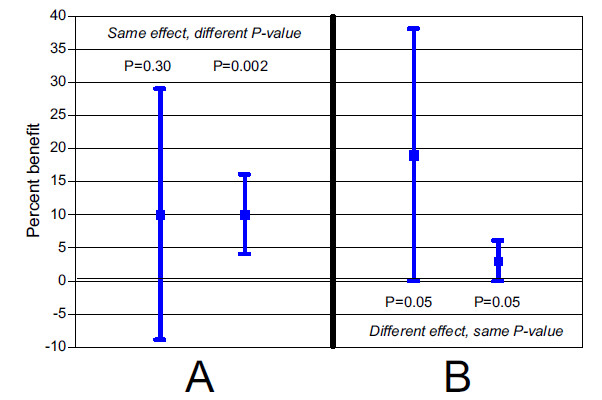
\includegraphics[width=0.5\textwidth,height=\textheight]{graphics/pValueEffectSize.jpg}

\vspace{2mm}

\scriptsize

Goodman (2008)

\flushleft
\normalsize

\(~\)

\textbf{Problem:} The \(p\)-value blands the estimated effect size with
its uncertainty.
\end{frame}

\begin{frame}
\begin{block}{Shall we abolish \(p\)-values?}
\protect\hypertarget{shall-we-abolish-p-values}{}
\(~\)

\centering


\includegraphics[width=0.6\textwidth,height=\textheight]{graphics/psycholog.png}

\flushleft
\vspace{6mm}

\begin{itemize}
\tightlist
\item
  But that throws the baby out with the bath water. It's as if we would
  forbid trains because they cannot fly to South America\ldots{}
\end{itemize}

\vspace{2mm}

\begin{itemize}
\tightlist
\item
  \(p\)-values are not ``good'' or ``bad''. They have \textbf{strengths}
  and \textbf{weaknesses}.
\end{itemize}
\end{block}
\end{frame}

\begin{frame}
\begin{block}{What should we do then?}
\protect\hypertarget{what-should-we-do-then}{}
\(~\)

\centering

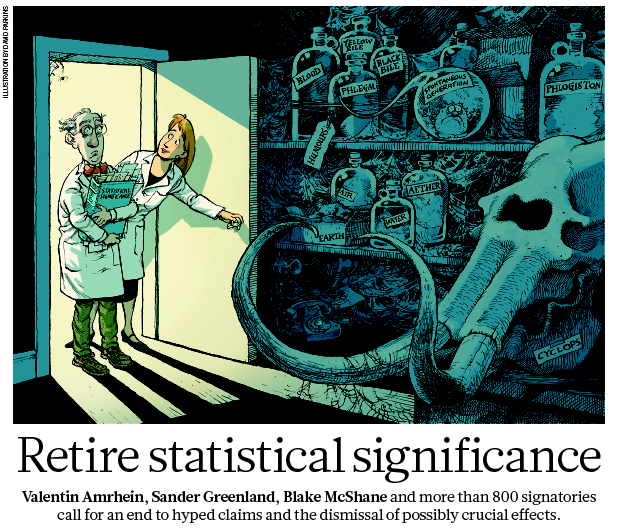
\includegraphics[width=0.5\textwidth,height=\textheight]{graphics/retire_significance.png}

\scriptsize

\normalsize

\(~\)

\flushleft

\begin{itemize}
\tightlist
\item
  In many situations it is not justified to make a strict yes/no
  decision.\footnote{\scriptsize And we are usually not forced to! In contrast to e.g. clinical trials.}
\end{itemize}

\vspace{2mm}

\begin{itemize}
\tightlist
\item
  \textbf{Instead}: accumulating evidence over more and more
  studies.\footnote{\scriptsize That's why it is so important to publish non-significant results, too! And: the importance of meta-analyses.}
\end{itemize}
\end{block}
\end{frame}

\begin{frame}
\begin{block}{A small literature review}
\protect\hypertarget{a-small-literature-review}{}
\(~\)

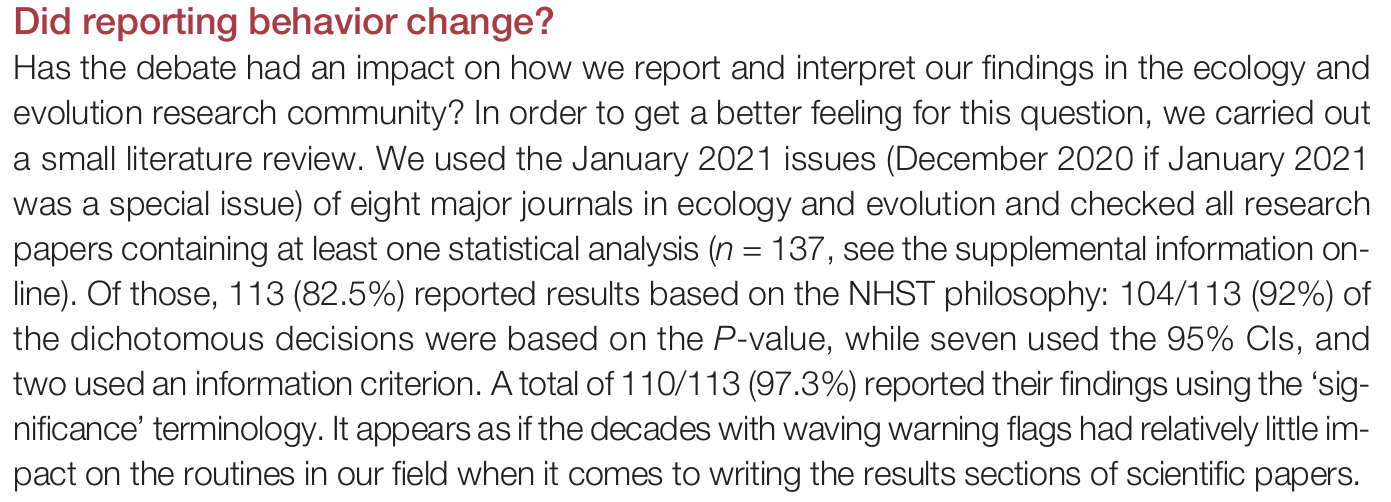
\includegraphics{graphics/reporting.png}
\end{block}
\end{frame}

\begin{frame}
\begin{block}{Suggestion 1: Language matters!}
\protect\hypertarget{suggestion-1-language-matters}{}
\vspace{2mm}

Rewrite your results and use a
\emph{\textcolor{red}{gradual interpretation of the $p$-value}}.

\vspace{2mm}

For single (observational) studies, the following has been suggested
already decades ago (Bland 1986):

\vspace{5mm}

\centering

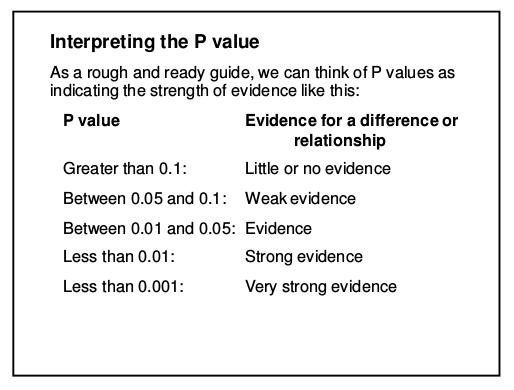
\includegraphics[width=0.6\textwidth,height=\textheight]{graphics/JMBland.png}
\end{block}
\end{frame}

\begin{frame}
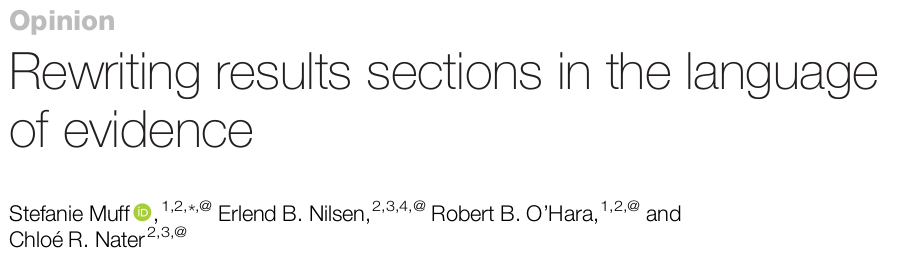
\includegraphics[width=1\textwidth,height=\textheight]{graphics/tree_title.png}
\(~\)

\centering

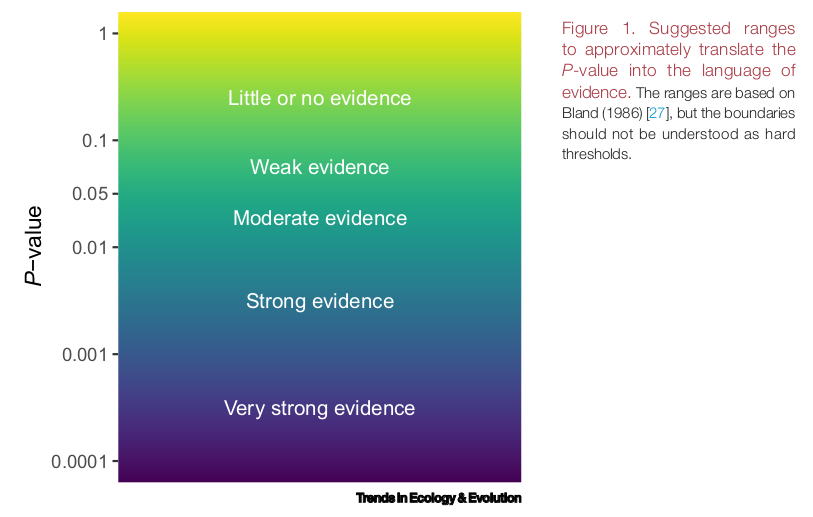
\includegraphics[width=0.7\textwidth,height=\textheight]{graphics/tree_figure.png}
\end{frame}

\begin{frame}
\begin{block}{Suggestion 2: Report effect sizes, 95\% CIs, and figures}
\protect\hypertarget{suggestion-2-report-effect-sizes-95-cis-and-figures}{}
\(~\)

Ask:

\vspace{2mm}

\begin{itemize}
\tightlist
\item
  Is the effect size (biologically, medically, socially\ldots) relevant?
\end{itemize}

\(~\)

\begin{itemize}
\tightlist
\item
  Which range of true effects is statistically consistent with the
  observed data?
\end{itemize}

\(~\) \centering \(\rightarrow\) 95\% confidence interval

\(~\)

\(~\)

\flushleft

\(~\)

\scriptsize

However

\(~\)

\begin{itemize}
\tightlist
\item
  The choice of the 95\% is again somewhat arbitrary. We could also go
  for 90\% or 99\% or any other interval.
\end{itemize}

\(~\)

\begin{itemize}
\tightlist
\item
  The 95\% CI should \textbf{not be misused for simple hypothesis
  testing} in the sense of ``Is 0 in the confidence interval or not?''
  -- that is just significance testing.
\end{itemize}
\end{block}
\end{frame}

\begin{frame}
A results table from an example where I was involved (Imo et al. 2018):

\centering

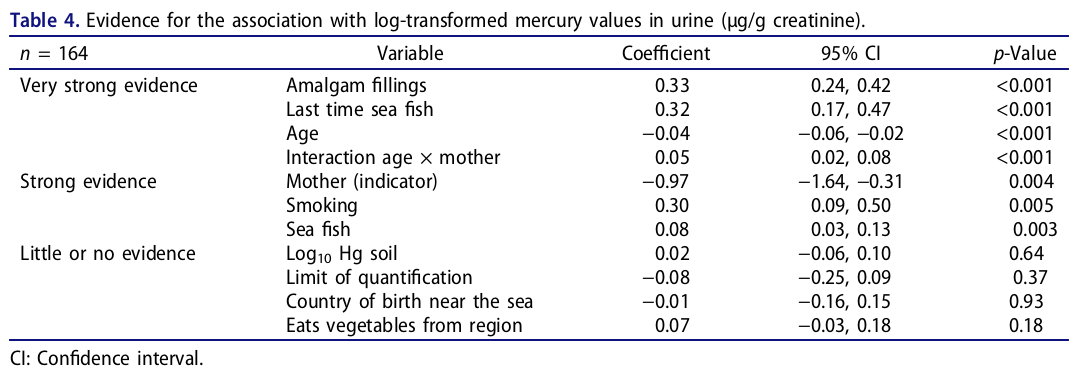
\includegraphics[width=0.8\textwidth,height=\textheight]{graphics/hg_table.png}

\(~\)

\begin{quote}
We found very strong evidence for a positive association of mercury in
urine with amalgam fillings (regression coefficient: 0.33; 95\% CI:
0.24--0.42; p \textless{} 0.001).
\end{quote}

\(~\)

\begin{quote}
We found no evidence for an association of log-transformed mercury
concentrations in soil with log-transformed concentrations in urine
(regression coefficient: 0.02; 95\% CI: −0.06--0.10; p = 0.64).
\end{quote}
\end{frame}

\begin{frame}
A graphical description often says more than thousand words\ldots{}

\(~\)

Do you prefer

\centering

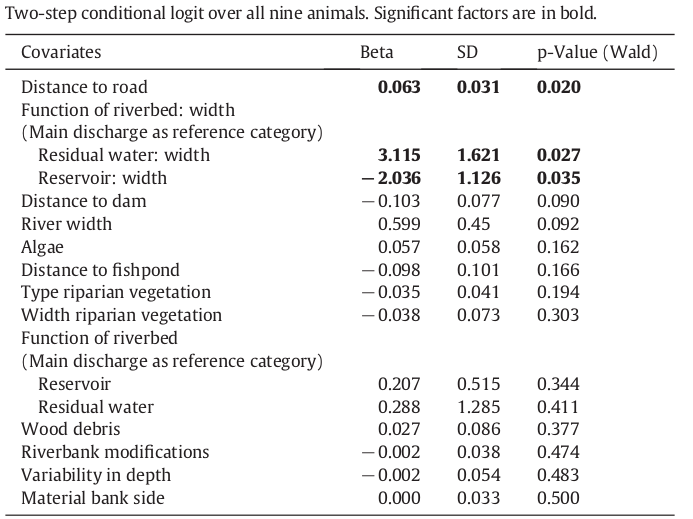
\includegraphics[width=0.6\textwidth,height=\textheight]{graphics/weinberger_table.png}
\end{frame}

\begin{frame}
or \ldots{} ?

\centering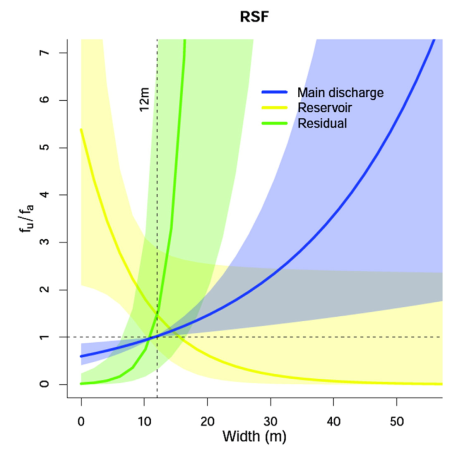
\includegraphics[width=0.6\textwidth,height=\textheight]{graphics/weinberger.png}

\(~\)

\flushleft
\scriptsize

(Weinberger et al. 2016)
\end{frame}

\begin{frame}
\begin{block}{The interpretation of the \(p\)-value depends!}
\protect\hypertarget{the-interpretation-of-the-p-value-depends}{}
\(~\)

\begin{itemize}
\tightlist
\item
  Observational vs experimental study
\end{itemize}

\vspace{2mm}

\begin{itemize}
\tightlist
\item
  Exploratory vs confirmatory analysis
\end{itemize}
\end{block}
\end{frame}

\begin{frame}
\begin{block}{Practice in drug regulation}
\protect\hypertarget{practice-in-drug-regulation}{}
\vspace{4mm}

Clinical trials (CTs) for \textbf{drug approval} underlie strict
requirements -- since decades.

\(~\)

\begin{itemize}
\tightlist
\item
  CTs are \textbf{randomized controlled trials}.
\end{itemize}

\vspace{2mm}

\begin{itemize}
\tightlist
\item
  \textbf{Study protocols} that are published even before any patient is
  treated.
\end{itemize}

\vspace{2mm}

\begin{itemize}
\tightlist
\item
  \textbf{Preregistration} of study protocols and analysis plans.
\end{itemize}

\vspace{2mm}

\begin{itemize}
\tightlist
\item
  \textbf{Two Trials Rule}:
\end{itemize}

\(~\)

\begin{quote}
\textcolor{orange}{"at least two adequate and well-controlled studies,
each convincing on its own, to establish effectiveness."}
\end{quote}

\(~\)

\(~\)
\end{block}
\end{frame}

\begin{frame}
\(~\)

\begin{itemize}
\tightlist
\item
  Clinical trials are \emph{experimental} and \emph{confirmatory}, and
  there are very strict regulations.
\end{itemize}

\(~\)

\begin{quote}
\textcolor{orange}{$\rightarrow$ We can draw a causal conclusion.}
\end{quote}

\vspace{4mm}

\begin{itemize}
\item
  On the other hand, in Ecology: (Often) observational studies, lots of
  researchers degrees of freedom, usually no preregistration,
  exploratory data analysis, no study protocols, model
  selection,\ldots{}

  \(~\)

  \begin{quote}
  \textcolor{orange}{$\rightarrow$ We are mostly detecting correlations.}
  \end{quote}
\end{itemize}

\(~\)
\end{frame}

\begin{frame}{Exercise}
\protect\hypertarget{exercise}{}
\(~\)

\begin{itemize}
\tightlist
\item
  Work in teams of 2-3 and choose one of the papers I will give you.
\end{itemize}

\(~\)

\begin{itemize}
\tightlist
\item
  Check how the authors reported their results.
\end{itemize}

\(~\)

\begin{itemize}
\tightlist
\item
  Make concrete suggestions (e.g., example sentences) how the authors
  could have better presented their results.
\end{itemize}

\(~\)

The material can be found here:

\url{https://github.com/stefaniemuff/statlearning/tree/master/OpenScience}
\end{frame}

\begin{frame}{``Homework''}
\protect\hypertarget{homework}{}
\(~\)

I recommend you to read the following short articles (you find the pdfs
on the literature list):

\(~\)

\begin{itemize}
\tightlist
\item
  Scientists rise up against statistical significance (2019). Amrhein et
  al., \emph{Nature}, 567, p.~305--307,
  \url{https://doi.org/10.1038/d41586-019-00857-9}
\end{itemize}

\vspace{2mm}

\begin{itemize}
\tightlist
\item
  The ASA statement on \(p\)-values: context, process, and purpose
  (2016). Wasserstein and Lazar, \emph{The American Statistician}, 70:2,
  129-133, \url{https://doi.org/10.1080/00031305.2016.1154108}
\end{itemize}

\vspace{2mm}

\begin{itemize}
\tightlist
\item
  Rewriting results sections in the language of evidence (2022). Muff et
  al., \emph{Trends in Ecology and Evolution}, 37, 203--210,
  \url{https://doi.org/10.1016/j.tree.2021.10.009}
\end{itemize}
\end{frame}

\begin{frame}{References}
\protect\hypertarget{references}{}
\scriptsize

\hypertarget{refs}{}
\begin{CSLReferences}{1}{0}
\leavevmode\vadjust pre{\hypertarget{ref-altman_bland1995}{}}%
Altman, D. G., and J. M. Bland. 1995. {``Absence of Evidence Is Not
Evidence of Absence.''} \emph{British Medical Journal} 311: 485.

\leavevmode\vadjust pre{\hypertarget{ref-amrhein.etal2019}{}}%
Amrhein, V., S. Greenland, and B. McShane. 2019. {``Retire Statistical
Significance.''} \emph{Nature} 567: 305--7.

\leavevmode\vadjust pre{\hypertarget{ref-bland_1986}{}}%
Bland, J. M. 1986. \emph{An Introduction to Medical Statistics}. Oxford:
Oxford Medical Publications.

\leavevmode\vadjust pre{\hypertarget{ref-goodman2008}{}}%
Goodman, S. N. 2008. {``A Dirty Dozen: Twelve {P}-Value
Misconceptions.''} \emph{Seminars in Hematology} 45: 135--40.

\leavevmode\vadjust pre{\hypertarget{ref-goodman2016}{}}%
---------. 2016. {``Aligning Statistical and Scientific Reasoning.''}
\emph{Science} 352: 1180--82.

\leavevmode\vadjust pre{\hypertarget{ref-imo.etal2018}{}}%
Imo, D., S. Muff, R. Schierl, K. Byber, Ch. Hitzke, M. Bopp, M. Maggi,
S. Bose-O'Reilly, L. Held, and H. Dressel. 2018. {``Human-Biomonitoring
and Individual Soil Measurements for Children and Mothers in an Area
with Recently Detected Mercury-Contaminations and Public Health
Concerns: A Cross-Sectional Study.''} \emph{Nternational Journal Of
Environmental Health Research} 28: 1--16.

\leavevmode\vadjust pre{\hypertarget{ref-ioannidis2005}{}}%
Ioannidis, J. P. A. 2005. {``Why Most Published Research Findings Are
False.''} \emph{PLoS Medicine} 2: e124.

\leavevmode\vadjust pre{\hypertarget{ref-nuzzo2014}{}}%
Nuzzo, R. 2014. {``Scientific Method: Statistical Errors.''}
\emph{Nature} 506: 150--52.

\leavevmode\vadjust pre{\hypertarget{ref-wasserstein.lazar2016}{}}%
Wasserstein, R. L., and N. A. Lazar. 2016. {``The {ASA}'s Statement on
p-Values: Context, Process, and Purpose.''} \emph{The American
Statistician}.

\leavevmode\vadjust pre{\hypertarget{ref-weinberger.etal2016}{}}%
Weinberger, I. C., S. Muff, A. Kranz, and F. Bontadina. 2016.
{``Flexible Habitat Selection Paves the Way for a Recovery of Otter
Populations in the {E}uropean {A}lps.''} \emph{Biological Conservation}
199: 88--95.

\end{CSLReferences}
\end{frame}

\end{document}
